\section{Compiler} \label{section:compiler}

The fluxionnal execution model is a framework to build distributed web applications, no better than so many already out.
This paper is about allowing any web application to run on this distributed execution model.

We want to enable parallelism in web applications.
To enable parallelism, we need to split a program into the many parts parallelisable.

Promises and Futures are abstractions for apparent synchronous program to run in an asynchronous fashion.
They abstract synchronous long waiting operation into asynchronous operation allowing an application to be parallelised, while conserving an imperative programming style.
This asynchronous shift allow parallelization because it creates a fork in the execution flow.
The execution will continue with the instructions that don't needs the waiting operation to complete, while the instructions that needs the operation to complete are just waiting for it.
This two execution paths could possibly run in parallel, because the two are made independent by the future or the promise : if one need the other, it simply waits for it to finish.
We call rupture points, the points where the execution flow forks in two distinct and parallelisable paths.

% Promises\cite{Liskov1988} describes a mechanism to replace RPCs in order to allow concurent parallelism in a distributed system.

% They argue that for performance concerns, are better because asynchronous, but harder for the developer to develop.
% So their solution is to provide a mechanism allowing asynchronism between the caller and the callee, with a promise about the result of this call for the caller to manipulate the result.

% Promises are about distributed system already, it's exactly like fluxions : a system to help the developer abstract parallelism in distributed system, without sacrificing performance.

% Futures allow parallelisation of evaluation in a programming language, by stopping processes that need a value not yet ready.

% message passing is better for performance, but call is better for human (see Promises: linguistic support for efficient asynchronous procedure calls in distributed systems).

% Promises and Futures are a synchronisation mechanism to abstract call into message passing.

Javascript is a functional and dynamically typed language initially introduced to handle user interactions within Web pages.
While Javascript isn't natively event-based, the DOM used in Web pages is.
The latter uses an event-loop to handle events happening on the Web page, and then triggers associated functions the developer provides.

More recently, \textit{Node.js} used the same event-loop based structure, to propose a non-blocking, event-based execution environment, specifically adapted for real-time I/O intensive applications like Web services.
Because of this event-loop based architecture, the I/O API \textit{Node.js} provides is non-blocking and asynchronous.
The invocation of any function from this API returns immediately not to block the execution with time consuming I/O operations.
The developer provide an handler function as argument for this asynchronous function to invoke when the operation completes.
This handler function is commonly named a callback, \textit{Node.js} uses the convention to place the callback as the last parameter.
The \textit{Node.js} event-loop receives and gathers every I/O event, waiting its turn in the loop to invoke the associated callback.
% Listing \ref{lst:callback} illustrates the call of the asynchronous function \texttt{asyncFn} with the callback \texttt{callbackFn}.

In most imperative languages the execution is synchronous by default, while special libraries handle parallelism, some using asynchronism like Promises\cite{Liskov1988} and Futures.
However, Node.js imposes natively both synchronous and asynchronous paradigms.
The asynchronicity of I/O Operations splits the execution and parallelize these two execution paths.

A rupture point is an asynchronous function call, defined by these two properties :
\begin{itemize}
 \item the function is asynchronous
 \item the function is of higher order
\end{itemize}

% \begin{code}[Javascript, caption={Example of an asynchronous function call},label={lst:callback}]
% function MyFn() { 
%   var a = 1,@\Comment{\circled{1}}@
%       b = 2,
%       c = 3;
%   asyncFn(a, b, function callbackFn(result) {
%     // process the result of asyncFn @\Comment{\circled{3}}@
%     // Use variables b, and c.
%   });
%   // result is not yet ready @\Comment{\circled{2}}@
% }
% \end{code}

% \begin{figure}[h!]
%   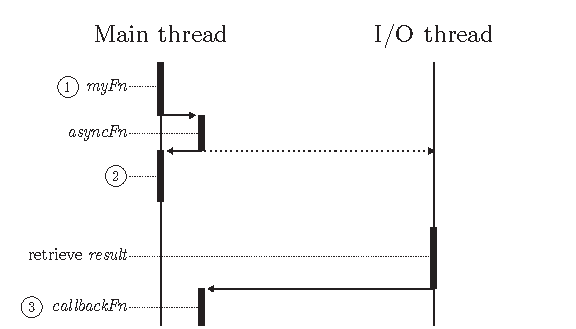
\includegraphics[width=\linewidth]{callback.pdf}
%   \caption{Illustration of listing \ref{lst:callback}}
%   \label{fig:callback}
% \end{figure}


The ruptures points mark out the parallelisables parts of a web application.
One of the compiler step, the pruner, spot the rupture points, and split the application along them.

But as long as the memory is shared, the application can't be distributed on multiple nodes.
The compiler need to split the shared memory into the application parts.

A function define its own scope, child of the function's scope the child function is defined within.
A child function can access every of its parent scope up to the root scope.
The root scope is called global, or window, wether you are in node.js or a browser.

In Javascript, the memory is enclosed in nested scopes, like russian dolls.
Each function create a new scope containing variables local to itself.
This scope is chained to the scope of the parent function, so that the child function can access the scope of the parent.
Callbacks defined inside a scope can access the same scope as the calling function, allowing them to share variables.
% This functionning is what allow closures : function acceding its parent scope, long after the parent finished its execution.

Rupture points define application parts along scopes frontier.
A scope is never shared two fluxions.
However, two nested scopes can be separated in two different fluxions.
As there is a root scope, parent of every scope, this root scope can't be in two different fluxions.
But childs scopes could be in different fluxions, thus, these childs wouldn't have access to the root scope variables, because encapsulated inside fluxions.
So variables from the parents would be made unavailable if the two scopes were spearated into two distributed application parts.
Another compiler step, the linker, understand and resolve dependenciy conflicts between the distributed functions scopes.



% ... to encapsulate them in fluxions, and migrate their execution onto different machines.
% Figure \ref{fig:callback} illustrates the two isolated parts encapsulated in fluxions from listing \ref{lst:callback}.

% \begin{figure}[h!]
%   \includegraphics[width=\linewidth]{callbackFlx.pdf}
%   \caption{Illustration of listing \ref{lst:callback} broken into fluxions}
%   \label{fig:callback}
% \end{figure}

In the next subsections, we describe the different compilation steps.
The compiler uses program from the community, they are described in the first subsection along with the first compilation step.
Then, we describe the two following, important compilation steps : the \textit{pruner} breaks a program into many independent parts and the \textit{linker} resolves inconsistencies in the shattered functions scopes.

% In the next subsections, we describe our work on a compiler to break a program into many independent parts and enclose them in fluxion.
% We then address the limitations of this method, and possible future improvements.

\subsection{Common Tools}

The first step for the compiler is to parse the source file to extract the semantic of the web application, and to produce a representation to work on.
Some tools exist to parse and analyze Javascript source code (Esprima, Acorn ...).
We use a serie of tool written by Ariya Hidayat and Yusuke Suzuki : Esprima, Estraverse, Escope, Escodegen.
These tools use the specification for an intermediate representation of the Javascript source code from the Mozilla Javascript Parser API : the Abstract Syntax Tree (AST)\footnote{\raggedright https://developer.mozilla.org/en-US/docs/Mozilla/Projects/SpiderMonkey/Parser\_API}.

This structured representation breaks the source into a tree of nodes, each representing a construct from the source, like an operation or an identifier.
It can be traversed and allow easy modification of its structure, without the risk of errors involved by direct source manipulation.

An example node in the AST is :

\begin{code}[Javascript, caption={Example of an AST node},label={lst:astnode}]
CallExpression {
    type: "CallExpression";
    callee: <Expression>;
    arguments: [ <Expression> ];
}
\end{code}

We use Esprima to parse the source and generate the AST.
We use Escope to detect function scope in this previously generated AST. 
We use Escodegen to print back AST into plain Javascript.
We use Estraverse to traverse and modify the AST.

\TODO what more here ?


\subsection{Pruner : breaking the program}

The pruner detect rupture points, breaking the program along them, and map every function scope to its corresponding fluxion.
Rupture points are calls of asynchronous function of higher order.
In an AST, the node of a function call is of type \textit{CallExpression}, and contains a reference to the callee and an array of the arguments.




We distinguish specials rupture points for asynchronous function handling series of external requests.
Unlike basic rupture points indicating a continuity in the execution flow.
The reception of an external request indicate a starting point in the execution flow.
These two types of rupture points corresond to different asynchronous functions in the \textit{Node.js} I/O API : the functions handling a series of I/O events, and the functions handling only one I/O event.

We distinguish these two types of rupture points to simplify later the system load dynamic analysis.
The system load is only dependent at run time of the input in the system, everything else can be infered before run-time.

\subsubsection{Series of events} \label{sss:start}

Some asynchronous functions provide a callback for a series of future event.
The handler of a network socket is called once for each incoming request.
The callbacks of these functions indicate the input of a data stream in the program, and the beginning of a fluxions chain.
As the callbacks mark the frontier between the current fluxion and the beginning fluxions chain, the compiler replaces the callback by a placeholder function starting the chain.
% This placeholder function uses the function \texttt{start(<msg)} provided by the fluxionnal execution model described section \ref{section:model}.
% The placeholder function is detailed later, section \ref{ss:Scope}.

\subsubsection{One-time event} \label{sss:post}

The other type of asynchronous functions provides immediate I/O operation.
Callbacks of these functions are invoked only once, and continue the execution after the completion of the I/O operation.
Because of their asynchronism, these function calls mark the frontier between the current fluxion and the next one, inside a chain of fluxion.
The compiler replaces the asynchronous function call by a call to a placeholder function.
% This placeholder function uses the function \texttt{post(<msg>)} provided by the fluxionnal execution model described section \ref{section:model}.
% The placeholder function is detailed later, section \ref{ss:Scope}.


The compiler detects rupture points with their type during the static analysis, with a dictionnary of asynchronous functions.

If the compiler detects the express module, a famous node.js web framework, it builds the dictionnary to detect later the variable declared for this module.
To find possible rupture points, the compiler tests the callee expression against this dictionnary for each callExpression node in the AST.

The compiler detects one rupture point for the following hello world program: 

\begin{code}[Javascript, caption={Hello World},label={lst:astnode}]
var app = require('express');
app.get('/', function(req, res) {
  res.send("Hello World :)");
});
\end{code}

% TODO insert the graph for this program

There is in this program only two scopes, the global scope, and the scope of the anonymous function.
These two scopes don't share any variable.


\begin{code}[Javascript, caption={Counter},label={lst:astnode}]
var app = require('express'),
    rep = "Hello World :)";
app.get('/', function(req, res) {
  res.send(rep);
});
\end{code}

In this slightly more complex programme, the two fluxion share a common variable : \texttt{rep}.
The pruner don't do anything to resolve this lacking dependency.
We see in the next subsection how this variable is handled by the linker.

\subsection{Linker} \label{ss:linker}


According to Brewer's theorem, formalized later by [??], a distributed application can only have two among the three options, Consistency, Availability, Partition tolerance.
Brewer said this article is "pretty good" http://codahale.com/you-cant-sacrifice-partition-tolerance/
Partition tolerance can't be avoided, a distributed system can't avoid to have failure.
So the only possible trade off is between consistency and availability.

In http://voltdb.com/blog/voltdb-products/clarifications-cap-theorem-and-data-related-errors/ Mike Stonebraker says that the trends is to make big data applications run on larger cluster of unreliable servers.
But his point in this article is to say that a 200 machines cluster with SQL is equivalent of a 4 machines custer with VoltDB, but 4 machines are less likely to crash.

As the trend is to use larger and larger cluster of commodity machines, transactional systems trading availability for consistency, will become slower and slower.
Choosing to sacrifice consistency might make more sense.
It let design a lot more flexible solution, which might have a better chance to cope with this kind of highly distributed architecture.

There exist solution to minimize the impact of error due to inconsistency.
Dynamo system : http://s3.amazonaws.com/AllThingsDistributed/sosp/amazon-dynamo-sosp2007.pdf




While walking the AST, the compiler register and track every use of variables to determine which ones and what type of access the fluxion needs, and which scope they belong to.
This set of variables needed by a fluxion represent its signature.
For example, the signature of the fluxion created out of \texttt{asyncFn}, listing \ref{lst:callback} include variables \texttt{b} and \texttt{c} as they are used in \texttt{callbackFn}, as well as \texttt{a} because it is used by the function call to \texttt{asyncFn}.
To resolve these dependencies, during the execution, the parent function sends the signature of the next fluxion in the same message together with the result of the asynchronous operation.
As the placeholder function call have the same scope than the asynchronous function call or callback it replaces, it is responsible for gathering the variables from the signature in a message along with the result of the operation and send it to the next fluxion.
The placeholder function call replacing \texttt{asyncFn} after compilation of listing \ref{lst:callback} is described in listing \ref{lst:placeholder}, line \ref{lst:placeholdercall}.

% \begin{code}[Javascript, caption={Example of a placeholder function call},label={lst:placeholder}]
% function MyFn() {
%   var a = 1,
%       b = 2,
%       c = 3;

%   // Placeholder for asyncFn-uid
%   flx.post(flx.m("asyncFn-uid", {a, b, c})); @\label{lst:placeholdercall}@
% }
% \end{code}



% Stream line
As fluxions are chained one after another, a fluxion must provide every dependency for the next one, even if some of this dependencies miss from its own scope or signature.
These dependencies must be passed fluxion after fluxion from the producing fluxion, to the consuming fluxion.
So, the message stream linking one fluxion to another includes the signature of the next fluxion as well as dependencies targeting downstream fluxions.
The compiler has to resolve the content of these message streams beginning by the last fluxions and going upstream to the first ones.
Figure \ref{fig:streamline} illustrate this principle : since fluxion \textit{C} needs the variable \textit{z}, fluxion \textit{B} needs the variable \textit{z} as well to pass it along to fluxion \textit{C}.

\begin{figure}[h!]
  \includegraphics[width=\linewidth]{ressources/streamline.pdf}
  \caption{Fluxion C needs the variable z, so does fluxion B}
  \label{fig:streamline}
\end{figure}

\subsection{Limitations} \label{ss:Limitations}

% For example, functions from the \texttt{Array} prototype ask functions as parameters for a behavior to call on each iteration over the array.
% Listing \ref{lst:array} presents an example of this structure.
% This iteration is synchronous, so the function passed as an argument, \circled{1}, and the code following the function call, \circled{2}, are somehow dependent.
Leaving an asynchronous function call as is doesn't introduce bugs, however breaking a synchronous function by replacing its callback leads to bugs.
To avoid introducing new bugs, it is important for the compiler to be able to distinguish between these synchronous and asynchronous functions.

% \begin{code}[Javascript, caption={Example of a synchronous function using a callback},label={lst:array}]
%   my_modified_array = my_array.map(function(element) {
%     // Modifying element @\Comment{\circled{1}}@
%   })
%   // Following code @\Comment{\circled{2}}@
% \end{code}

% Problem with dynamically typed functions

% Functions are of higher order in Javascript, so arrays can contain functions, as well as a variables.
Javascript is dynamically typed, if the index to access an array can't be resolved statically, then so do the type of the result.
Some callbacks can't be resolved statically.
For example, in listing \ref{lst:unresolved}, the function \texttt{myAsyncFn} is asynchronous and ask for a callback as parameter.
The compiler would break the program along its call, however \texttt{event.type} is unresolvable statically, the compiler is unable to include the callback in the next fluxion.
This structure might already be encapsulated inside a fluxion, and the callback might need variables from the scope of an upstream fluxion, but as the callback is unresolved, it is impossible for the compiler to track them, and add these dependencies in the signature of the current fluxion.
Even if the compiler leaves this structure as is, it introduce dependency bugs as the compiler is unable to resolve dependencies and generate accurate signatures.
The compiler is currently unable to compile a program containing structures involving dynamic resolution like in listing \ref{lst:unresolved}.

\begin{code}[Javascript, caption={Example of an unresolvable callback},label={lst:unresolved}]
myHandlers = [];
// ... definition of myHandlers
onEvent(function(event) {
  myAsyncFn(myHandlers[event.type])
})
\end{code}


\subsection{Futur Works}

Even synchronous, the use of a callback by the \texttt{map} function indicate an independence between the callback and the main execution thread.
For future improvements, we focus on studying these independences to allow the compiler to spot and break into fluxions these patterns of synchronous function call using callbacks.

For future improvements, we focus on a solution to dynamically compile fluxions and resolve dependencies, allowing to compile programs containing dynamic structures described in the last paragraph.

% \subsection{Compilation example}

% As of today our work on the compiler is still incomplete, there is inconsistencies between the high-level language detailed in section \ref{section:model} and the compilation results.
% For documentation purposes, this section details the compiler current state of progress.

% Listing \ref{lst:compsource} is a simplified version of the example listing \ref{lst:classique} in section \ref{section:model}.
% We use this simplified version as a test for our compiler, as it is yet unable to handle dynamic resolution, like used with the object \texttt{count} line \ref{lst:classique_dynres} in listing \ref{lst:classique}.
% The result of this compilation is listing \ref{lst:comptarget}.
% In the compilation result, the fluxion \textit{id-1000} should hold a context containing the variable \texttt{count}, like the object \texttt{uid} in the context of fluxion \textit{logic}, listing \ref{lst:fluxionnal}.
% But our compiler is yet unable to correctly resolve dependencies and fluxion contexts, so this counter service is unable to increment visits.

% \begin{code}[Javascript, caption={Simplified version of the initial service},label={lst:compsource}]
% var app = require('express')();
% var count = 0;

% app.get("/:id", function id(req, res){
%   count = count + 1;
%   res.send(count);
% });

% app.listen(8080);
% \end{code}

% \begin{code}[Javascript, caption={Compilation result of code listing \ref{lst:compsource}},label={lst:comptarget}]
% // Main >> id
%   var flx = require('fluxion');
%   var app = require('express')();
%   var count = 0;
 
%   app.get("/:id"n function placeholder(req, res) {
%     flx.start(flx.message("id-1000", {
%       res: res,
%       count: count
%     }))
%   })
 
%   app.listen(8080);

% // id-1000
%   flx.register("id-1000", function id-1000(msg){
%     res.send(msg.count = msg.count + 1);
%   })
% \end{code}





